%Dokumenteigenschaften
\documentclass[a4paper, 12pt]{article}
%import
\usepackage{blindtext}
\usepackage{hyperref}
\usepackage{pdfpages}
\usepackage{amsmath}
\usepackage{amssymb}
\usepackage[b]{esvect}
\hypersetup{linktoc=all}

\begin{document}
	%Titelseite
	\begin{titlepage}
		\title{\Large{\textbf{\underline{Simulation von Boids}}}\linebreak\large\textbf{nach Craig Reynolds}}
		\author{Oliver Fritzler}
		\date{\today}
		\maketitle
	\end{titlepage}

	%Inhaltsverzeichnis
	\title{\Large{\textbf{\underline{Inhaltsverzeichnis}}}}
	\tableofcontents
	%UML-Diagramm
	\section{UML-Diagramm}
	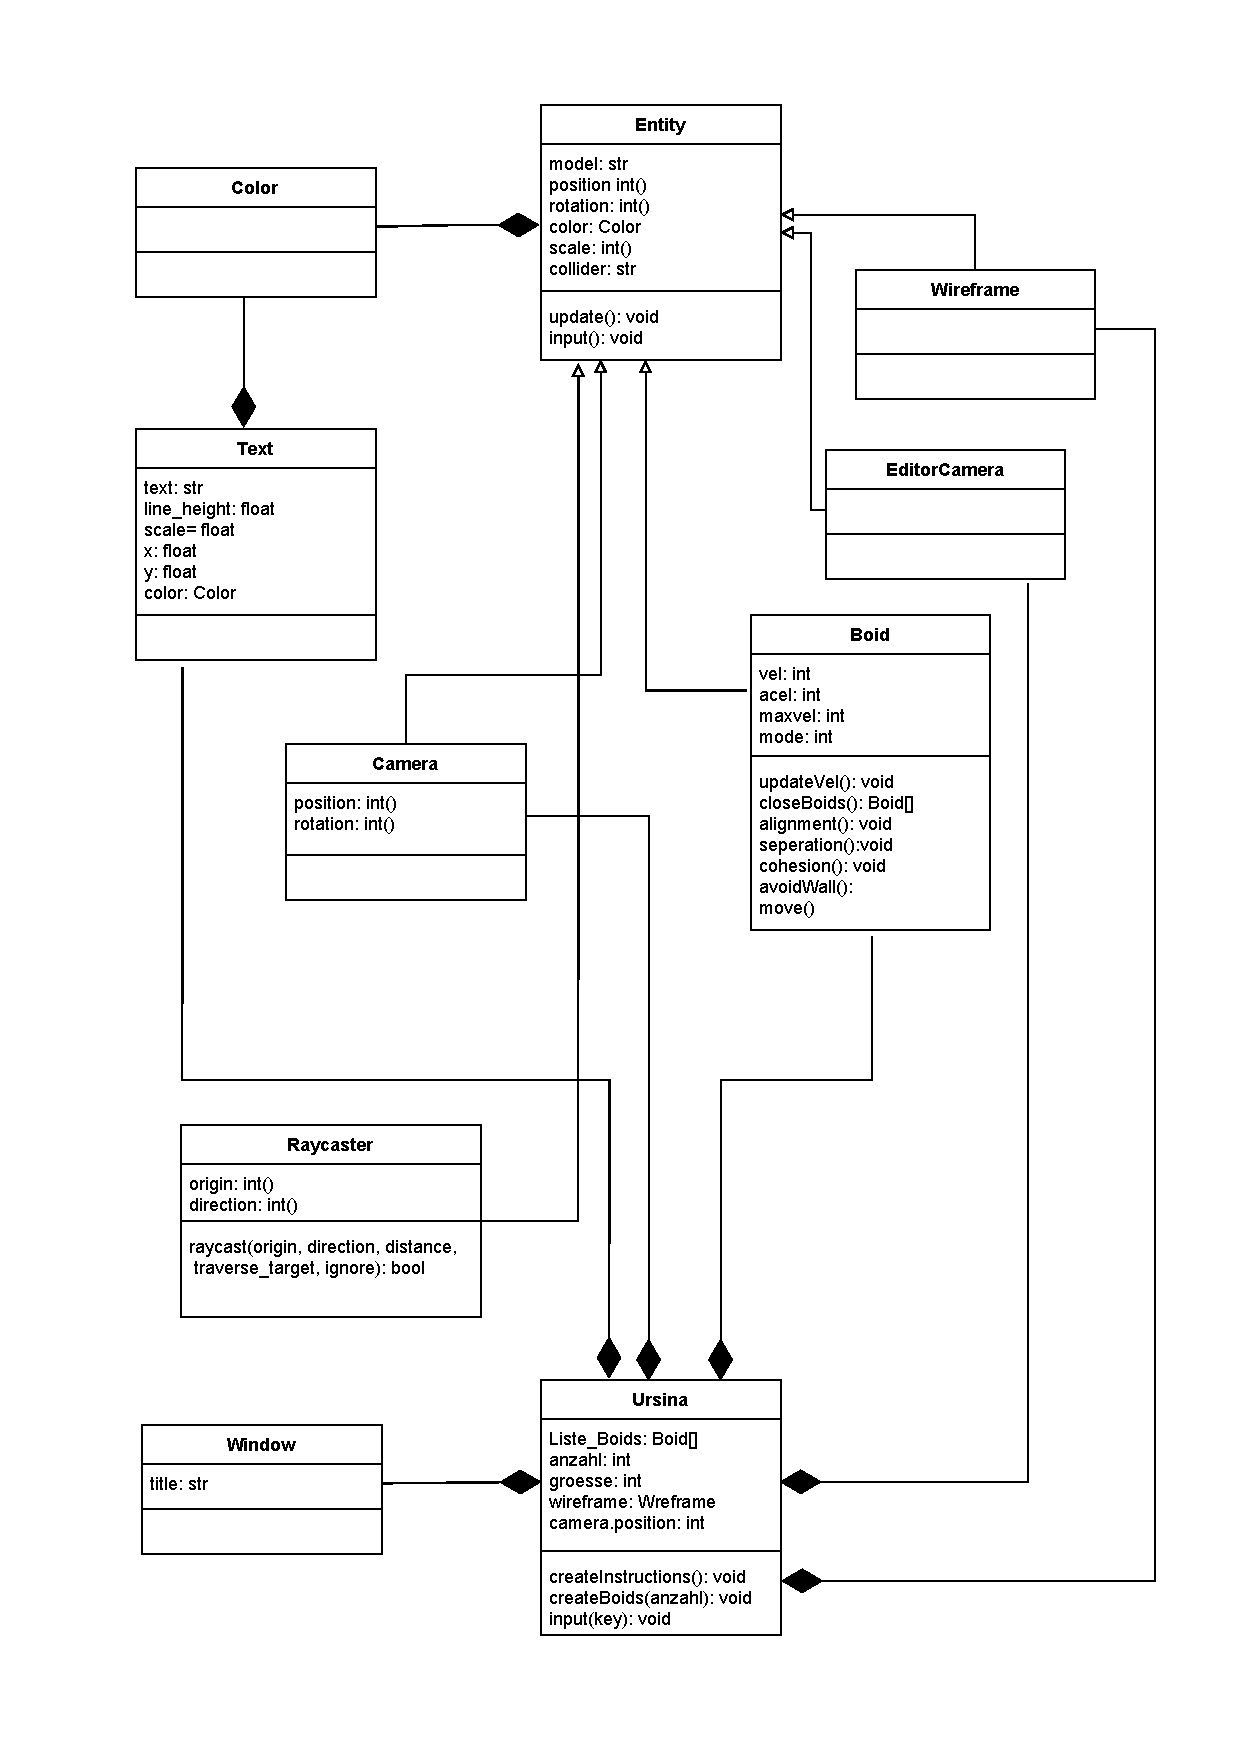
\includegraphics[scale=0.75, page=1]{UML/Boids_UML.pdf}
	\newpage
	%Grundidee
	\section{Grundidee}
	\subsection{Umgebung}
		Die Programmiersprache \emph{\textbf{Python}} war vorgegeben, die Bibliothek zur grafischen Darstellung war frei überlassen. Aufgrund der einfachen und verständlichen Syntax, fiel die Auswahl auf die \emph{\textbf{ursina engine}}, welche auf der \emph{\textbf{panda3D engine}} basiert. Ursina ermöglicht es neben vorgegebenen Modellen auch blender-Dateien als Modelle für die einzelnen Objekte zu verwenden. Diese Objekte werden dargestellt und durch spezifische Funktionen (update(), move()) jedes Bild aktualisiert. Dadurch kann man sowohl die Position durch Addition verändern, als auch Eingaben des Benutzers verarbeiten. 
	
	\subsection{Darstellung des Raumes}
		Zur Darstellung des Raumes werden 12 Objekte in Form eines Würfels erstellt, jedoch werden diese dann so skaliert, dass sie die Form eines Rechteckes annehmen. Diese werden dann so angeordnet, dass sie die Kanten eines Würfels bilden. 
		Des Weiteren werden die Seitenflächen erstellt. Dabei werden wie davor 6 Objekte in Form eines Würfels erstellt. Nur werden diese jetzt so skaliert, dass sie eine quadratische Fläche bilden. Um diese unsichtbar zu machen wird der Sichtbarkeitswert $\alpha$ auf Null gesetzt.
		
	\subsection{Allgemeines zu den Boids}
		Boids sind Körper, die sich Bewegen. Zur Veranschaulichung der Richtung sollten die Boids einen Körper mit einer Spitze haben, wie zum Beispiel ein Kegel. Da ein Kegel sehr viele Seiten hat, die alle jedes Bild berechnet werden müssen und dadurch die Performance senken, sollte man auf einen einfacheren Körper mit Spitze zurückgreifen, wie eine Pyramide.  Diese Körper bewegen sind jedoch nicht chaotisch, da sie sich an drei Regeln handeln, die später erklärt werden.\linebreak
		\newpage
		\textbf{\underline{Verhalten an Wänden}}
		Das Verhalten der Boids an den Wänden kann man auf verschiedene Weise gestalten. In dieser Simulation wurden drei davon versucht umzusetzen. 
		\begin{enumerate}
			\item \underline{\textbf{Warp}}\linebreak
			Bei dieser Umsetzung werden die Boids bei Kontakt mit einer Wand auf die gegenüberliegende Seite teleportiert.
			
			\item \underline{\textbf{Wände vermeiden}}\linebreak
			Dabei drehen die Boids vor Kontakt mit einer Wand ab.
			
			\item \underline{\textbf{Pong}}\linebreak
			Hier verhalten sich die Boids, wie der Ball im Spiel \textbf{"PONG"}, d.h. sie bewegen sich auf die Wand in einem bestimmten Winkel zu und verlassen diese Wand dann in dem gleichen Winkel, nach dem \emph{Einfallswinkel-gleich-Ausfallswinkel-Prinzip}
		\end{enumerate}

	\subsection{Regeln}
	Boids sind Objekte die sich in einem Raum bewegen. Dabei verfolgen sie drei Grundregeln:
	\begin{itemize}
		\item\textbf{\underline{Seperation}}\linebreak
		Diese Regel besagt, dass jeder einzelne Boid versucht, keinen anderen Boid zu treffen. 
		\item\textbf{\underline{Alignement}}\linebreak
		Diese Regel besagt, dass jeder Boid versucht, in die selbe Richtung wie ein anderer sich zu bewegen. Dadurch entsteht ein sogenannter "Flock" also ein Schwarm von Boids.
		\item\textbf{\underline{Coheseion}}\linebreak
		Diese Regel besagt, dass die Boids in die Mitte des Schwarms steuern.
	\end{itemize}
	
	\subsection{Eingabe}
	Der Benutzer soll durch Bewegen der Maus die Kamera rotieren können und durch Tastendruck die Kamera bewegen können. Außerdem soll es ihm ermöglicht werden die Anzahl der Boids und deren Verhalten zu ändern.
	\newpage
	
	
	
	\section{Umsetzung}
	\subsection{Fenster}
	Mit dem Aufrufen der Klasse \textbf{\emph{Ursina}} wird ein Fenster erschaffen, welches am Ende ausgeführt wird, mit all den benötigen Grafiken. Diesem Fenster kann man einen Titel vergeben, welche dann als Task angezeigt wird. Diese Klasse hat wie jede andere Klasse in Ursina die Funktion \textbf{\emph{input()}} mit deren Hilfe man die Eingabe des Benutzers verarbeiten kann, die in dieser Umsetzung hier nachzulesen sind. Um dem Benutzer die Nutzung der Simulation zu vereinfachen, erstellt man in der Funktion \textbf{\emph{createinstruction()}}, mit der Klasse \textbf{\emph{Text}} eine Beschreibung und skaliert und positioniert sie so, dass sie nicht im Vordergrund liegt.[Code]
	\subsection{Raum}
	In der Funtkion \textbf{\emph{createwireframe()}} werden 12 Objekte der Klasse \emph{\textbf{Entity}} in Form eines Würfel erstellt, die so verformt werden, dass sie zu Quadern werden und so positioniert werden, dass sie die Kanten eines größeren Würfels bilden. Darauf werden wie zuvor 6 Würfel erstellt, jedoch werden diese so skaliert, dass sie zu quadratischen Flächen werden, welche nach der Positionierung die Seitenfläche des Würfels bilden. Da diese Seiten nicht nötig zu sehen sind, kann der 4. Faktor der Farbe auf 0 gesetzt werden oder die Variable $\alpha$, die den Sichtbarkeitswert darstellt, auf 0 gesetzt wird. Bei dieser Umsetzung wird letzteres benutzt.[Code]
	
	\subsection{Boids}
	
	\subsection{Eingabe}
	%wichtigste Funktionen
	\newpage
	\section{wichtigste Funktionen}
	\newpage
	%Abbildungsverzeichnis
	\section{Abbildungsverzeichnis}
	\newpage
	%Quellennachweis
	\section{Quellennachweis}
	\newpage
\end{document}
